\documentclass[lettersize,journal]{IEEEtran}
\usepackage{rotating}
\makeatletter
\setlength{\@fptop}{0pt}
\makeatother
\usepackage{amsmath,amsfonts}
\usepackage{algorithmic}
\usepackage{algorithm}
\usepackage{array}
\usepackage[caption=false,font=normalsize,labelfont=sf,textfont=sf]{subfig}
\usepackage{textcomp}
\usepackage{stfloats}
\usepackage{url}
\usepackage{verbatim}
\usepackage{graphicx}
\usepackage{cite}
\hyphenation{op-tical net-works semi-conduc-tor IEEE-Xplore}
\def\BibTeX{{\rm B\kern-.05em{\sc i\kern-.025em b}\kern-.08em
    T\kern-.1667em\lower.7ex\hbox{E}\kern-.125emX}}
\usepackage{balance}
% updated with editorial comments 8/9/2021

\begin{document}

\title{Enhancing Molecular Generation with\\FragGPT-Guided Genetic Algorithms}

\author{Tiangai Yao, Zhangfan Yang, Junkai Ji,~\IEEEmembership{Member,~IEEE}\\
        % <-this % stops a space
\thanks{T. Yao, Z. Yang, and J. Ji are with the College of Computer Science and Software Engineering, Shenzhen University, Shenzhen 518060, China (e-mail: 2400671005@mails.szu.edu.cn; yangzhangfan@szu.edu.cn; jijunkai@szu.edu.cn).}% <-this % stops a space
\thanks{Manuscript received December 15, 2024; revised January 20, 2025.}}
% The paper headers
\markboth{IEEE Transactions on Evolutionary Computation,~Vol.~XX, No.~X, Month~2025}%
{Yao \MakeLowercase{\textit{et al.}}: Enhancing Molecular Generation with FragGPT-Guided Genetic Algorithms}

\IEEEpubid{1089-778X/25\$31.00~\copyright~2025 IEEE}
% Remember, if you use this you must call \IEEEpubidadjcol in the second
% column for its text to clear the IEEEpubid mark.

\maketitle
%摘要
\begin{abstract}
De novo molecular design poses a significant challenge in drug discovery, necessitating a delicate balance between exploring vast chemical spaces and targeting promising regions for optimization. This paper introduces FragGPT-GA, a novel hybrid evolutionary framework that synergistically combines a Genetic Algorithm (GA) with a Generative Pre-trained Transformer (GPT) to address this challenge. The core of our approach lies in using the GA for fine-grained structural optimization, while leveraging a fragment-based GPT model as an intelligent diversity generation operator. Specifically, the GPT model generates novel molecular candidates from masked fragments of the parent population, injecting high-quality and diverse individuals into the evolutionary loop. This mechanism enhances the exploratory capabilities of the GA, effectively preventing premature convergence to local optima. We demonstrate through comprehensive experiments, targeting a specific protein, that FragGPT-GA significantly outperforms traditional GA-only baselines in the generation of molecules with superior docking scores, drug-likeness (QED), and synthetic accessibility (SA). Our framework provides a powerful and robust strategy for efficient molecular discovery and optimization. 
\end{abstract}

\begin{IEEEkeywords}
Evolutionary Computation, Genetic Algorithm, Generative Pre-trained Transformer (GPT), De Novo Drug Design, Molecular Optimization, Hybrid Intelligence.
\end{IEEEkeywords}

\section{Introduction}
\IEEEPARstart{D}{e} novo drug design, the computational generation of novel molecules with desired pharmacological properties, is a cornerstone of modern pharmaceutical research. The sheer size of the chemical space, estimated to be larger than $10^{60}$ molecules, makes exhaustive search infeasible. Therefore, intelligent search strategies are paramount.

Evolutionary Algorithms (EAs), particularly Genetic Algorithms (GAs), have been widely applied to molecular optimization tasks. They excel at exploiting promising regions of the chemical space through operators like crossover and mutation. However, GAs often suffer from a loss of population diversity, leading to premature convergence and limiting their ability to discover truly novel molecular scaffolds.

On the other hand, deep generative models, such as Generative Pre-trained Transformers (GPTs), have shown remarkable success in learning the underlying distribution of chemical data and generating diverse and valid molecules. Their strength lies in exploration. However, guiding these models to generate molecules optimized for multiple, specific objectives (e.g., high binding affinity and good ADMET properties) remains a significant challenge.

% 添加雷达图
\begin{figure}[!t]
\centering
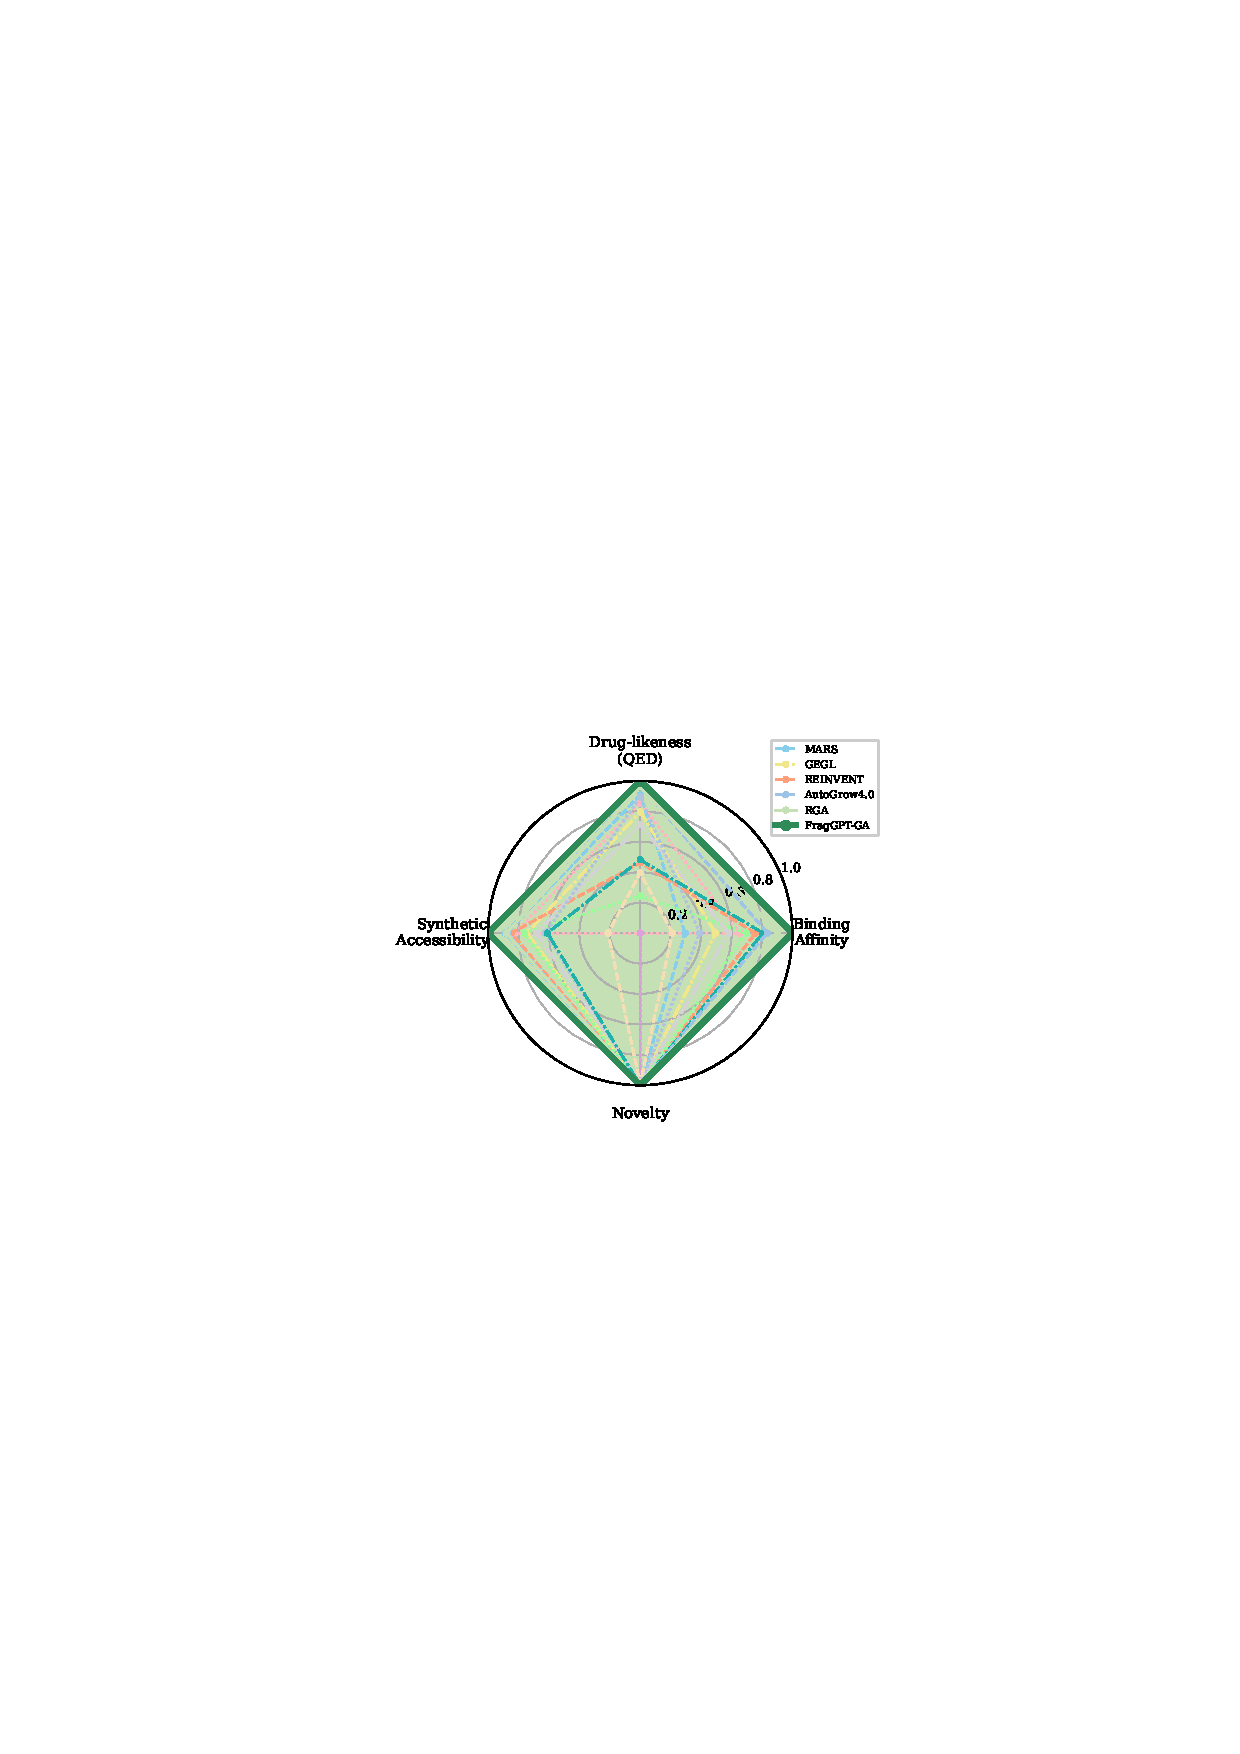
\includegraphics[width=2.5in]{paper_radar_chart.png}
\caption{Multi-objective performance comparison across key baseline methods. FragGPT-GA demonstrates superior performance with better balance across all metrics: binding affinity, drug-likeness (QED), synthetic accessibility, and novelty. The radar chart illustrates that FragGPT-GA achieves the best overall performance profile compared to RGA, AutoGrow4.0, and MARS baselines.}
\label{fig:radar_comparison}
\end{figure}

\IEEEpubidadjcol 
This paper addresses the limitations of both approaches by proposing a tightly-coupled hybrid framework, FragGPT-GA. As illustrated in Fig.~\ref{fig:radar_comparison}, our approach achieves superior performance with better balance across multiple objectives, demonstrating the best overall performance profile compared to existing baseline methods. We bridge the gap between exploration and exploitation by integrating a fragment-based GPT directly into the GA's evolutionary cycle. Our main contributions are:
\begin{enumerate}
    \item We propose the FragGPT-GA framework, a novel hybrid algorithm that synergizes a GA's optimization power with a GPT's diversity generation capabilities for molecular design.
    \item We introduce a unique mechanism where a GPT acts as an intelligent "diversity infusion" operator, generating new candidates from masked molecular fragments of the current population at each generation.
    \item We conduct extensive experiments demonstrating that FragGPT-GA achieves state-of-the-art performance in generating high-quality molecules compared to baseline methods.
\end{enumerate}
%相关工作
\section{Related Work}

De novo molecular design has emerged as a cornerstone of computational drug discovery, with various methodologies addressing the challenge of navigating vast chemical spaces to identify molecules with desired pharmacological properties. This section systematically reviews the evolutionary landscape of molecular optimization approaches, categorizing them by their core computational paradigms and analyzing their respective strengths and limitations.

\subsection{Evolutionary Algorithms in Molecular Optimization}

Evolutionary algorithms (EAs) have established themselves as robust optimization frameworks for molecular design, leveraging population-based search strategies to explore chemical space systematically. Traditional genetic algorithms encode molecules using string representations such as SMILES or graph-based structures, evolving populations through selection, crossover, and mutation operators guided by fitness functions derived from docking scores, bioactivity predictions, or multi-objective criteria.

\noindent \textbf{Classical Genetic Approaches:} Early implementations like Graph-GA \cite{jensenGraphBasedGeneticAlgorithm2019} operate directly on molecular graph representations, employing specialized crossover and mutation operators designed for graph structures. These methods demonstrate computational efficiency through parameter-free designs but suffer from limited exploration diversity. Similarly, traditional GA frameworks often implement chemically-aware heuristics such as BRICS-guided edits and reaction-based mutations to maintain chemical validity and synthesizability.

\noindent \textbf{Enhanced Evolutionary Strategies:} More sophisticated approaches integrate neural network guidance to address exploration limitations. The GA+D framework \cite{nigamAugmentingGeneticAlgorithms2020} augments genetic optimization with discriminator networks, employing SELFIES molecular representation to guarantee chemical validity while using neural networks to guide the evolutionary process. However, these discriminator-based approaches often require extensive hyperparameter tuning and may introduce computational overhead that limits scalability.

\noindent \textbf{Limitations of Pure Evolutionary Approaches:} Despite their optimization prowess, vanilla genetic algorithms suffer from fundamental limitations: (1) \textit{diversity collapse} - populations tend to converge prematurely around local optima, reducing scaffold novelty; (2) \textit{mode-seeking behavior} - the selection pressure often drives populations toward similar chemical motifs, limiting exploration of diverse chemotypes; (3) \textit{limited generative capacity} - traditional crossover and mutation operators struggle to introduce genuinely novel structural patterns beyond local modifications of existing molecules.

\subsection{Deep Generative Models for Molecular Design}

The advent of deep learning has revolutionized molecular generation, with various generative modeling paradigms demonstrating remarkable capabilities in learning chemical distributions and sampling novel molecular structures.

\noindent \textbf{Autoregressive and Variational Models:} Junction Tree Variational Autoencoders (JTVAE) \cite{jinJunctionTreeVariational2018} decompose molecules into chemically meaningful substructures, enabling structured generation while maintaining chemical validity. These approaches excel at capturing local chemical patterns but often struggle with long-range dependencies and complex multi-ring systems.

\noindent \textbf{Reinforcement Learning Approaches:} REINVENT \cite{olivecronaMolecularDeNovoDesign2017} employs recurrent neural networks for SMILES-based generation through reinforcement learning paradigms, demonstrating the ability to optimize molecules toward specific objectives. However, these methods face challenges in balancing exploration and exploitation, often requiring careful reward engineering and suffering from training instability. More sophisticated approaches like MolDQN \cite{zhouOptimizationMolecularRep2019} formulate molecular design as sequential decision-making processes using Markov Decision Process principles, but they struggle with sample efficiency and may converge to suboptimal solutions.

\noindent \textbf{Multi-Objective Generation:} Advanced frameworks address multi-objective optimization challenges. RationaleRL \cite{jinMultiObjectiveMoleculeGeneration2020} implements policy gradient optimization through message-passing neural networks for molecular graph generation, incorporating interpretable substructures. MARS \cite{xieMARS2021} executes Markov Chain Monte Carlo sampling with temperature annealing schemes for multi-objective molecular discovery, utilizing graph neural networks for proposal generation.

\noindent \textbf{3D-Aware Generation:} Recent developments include 3D structure-aware approaches like Gen3D \cite{luoGraph2022}, which generates molecules considering three-dimensional constraints for structure-based drug design. While promising, these methods often require extensive computational resources and may struggle with complex binding pocket geometries.

\noindent \textbf{Limitations of Pure Generative Approaches:} Despite impressive generative capabilities, deep learning models face significant challenges: (1) \textit{objective steering difficulty} - directing generation toward multi-objective optima (e.g., simultaneous optimization of binding affinity, drug-likeness, and synthetic accessibility) remains non-trivial; (2) \textit{sample inefficiency} - reinforcement learning-based approaches often require extensive sampling to achieve convergence; (3) \textit{training instability} - policy gradient methods and adversarial training can be unstable, leading to mode collapse or poor convergence; (4) \textit{limited exploitation} - purely generative approaches lack the systematic exploitation capabilities of evolutionary algorithms.

\subsection{Hybrid and Multi-Strategy Approaches}

Recognizing the complementary strengths of evolutionary and generative paradigms, recent research has explored hybrid methodologies that combine multiple optimization strategies.

\noindent \textbf{Loose Coupling Strategies:} Early hybrid approaches typically employ loose coupling mechanisms, such as initializing GA populations with generative models or periodically reseeding populations with neural proposals. While these methods demonstrate some improvement over individual approaches, they often underutilize model priors and may disrupt established GA dynamics.

\noindent \textbf{Guided Exploration Methods:} GEGL \cite{ahnGuidingDeepMolecular2020} represents a more sophisticated approach, guiding deep molecular optimization with genetic exploration. However, this method faces challenges in maintaining the balance between genetic algorithm rigour and neural network flexibility, often requiring extensive hyperparameter optimization.

\noindent \textbf{Current Limitations of Hybrid Approaches:} Existing hybrid methodologies suffer from several key limitations: (1) \textit{integration depth} - most approaches implement shallow integration, failing to leverage the full potential of both paradigms; (2) \textit{dynamic balance} - maintaining optimal balance between exploration (generative) and exploitation (evolutionary) components throughout optimization remains challenging; (3) \textit{computational efficiency} - combining multiple complex algorithms often results in significant computational overhead; (4) \textit{objective coordination} - ensuring that both generative and evolutionary components work toward consistent multi-objective goals is non-trivial.

\subsection{Fragment-Based Molecular Design}

Fragment-based approaches have gained prominence in both traditional medicinal chemistry and computational drug design, leveraging the principle that complex molecules can be decomposed into smaller, chemically meaningful building blocks.

\noindent \textbf{Traditional Fragment Approaches:} Classical fragment-based drug design relies on identifying small molecular fragments that bind to target proteins, subsequently linking or growing these fragments into larger, more potent compounds. This approach has proven successful in medicinal chemistry but often requires extensive manual intervention and domain expertise.

\noindent \textbf{Computational Fragment Methods:} Recent computational approaches have attempted to automate fragment-based design, using techniques such as BRICS decomposition to break molecules into chemically sensible fragments. However, these methods often struggle with fragment recombination and may generate chemically implausible structures.

Our FragGPT-GA framework addresses the limitations of existing approaches through several key innovations: (1) \textit{tight integration} - we implement deep integration between fragment-based GPT generation and genetic algorithm optimization, where the GPT operates as an intelligent diversity operator within the GA loop; (2) \textit{dynamic masking} - our approach employs dynamic fragment masking that adapts exploration intensity throughout the optimization process; (3) \textit{multi-objective coordination} - both generative and evolutionary components are coordinated toward consistent multi-objective goals through NSGA-II selection; (4) \textit{chemical validity preservation} - the fragment-based GPT approach ensures high chemical validity while maintaining synthetic accessibility.



% III. 方法 (The Proposed FragGPT-GA Framework)
% ----------------------------------------------------
\section{The Proposed FragGPT-GA Framework}

\subsection{Framework Overview and Design Philosophy}

The FragGPT-GA framework represents a paradigm shift in molecular optimization by establishing a tight integration between evolutionary algorithms and generative AI models. Unlike existing hybrid approaches that employ loose coupling strategies, our framework embeds a fragment-based GPT model as an intelligent diversity operator directly within the genetic algorithm's iterative loop. This deep integration enables the system to maintain the systematic optimization capabilities of evolutionary algorithms while leveraging the generative power and learned chemical knowledge of large language models.

The core innovation lies in treating the GPT model not as an external generative component, but as an adaptive operator that intelligently expands the search space based on the current population's genetic material. This approach addresses the fundamental limitation of traditional GAs—diversity collapse—while maintaining the directed optimization pressure essential for convergence to high-quality solutions.

\subsection{Architectural Components and Workflow}

The FragGPT-GA framework operates through a sophisticated multi-stage iterative process, as depicted in Fig.~\ref{fig:flowchart}. Each generation cycle encompasses five interconnected phases: (1) \textit{fragment-based molecular decomposition}, (2) \textit{intelligent GPT-driven diversity generation}, (3) \textit{population-aware genetic operations}, (4) \textit{multi-objective fitness evaluation}, and (5) \textit{Pareto-optimal selection}. This design ensures that exploration and exploitation are balanced dynamically throughout the optimization process.

% 流程图
\begin{figure}[!t]
\centering
\includegraphics[width=3.5in]{model_pictures_01.png}
\caption{The iterative workflow of the proposed FragGPT-GA framework. The process synergizes a Genetic Algorithm (GA) for optimization with a Generative Pre-trained Transformer (GPT) for diversity expansion, featuring dynamic fragment masking and multi-objective selection.}
\label{fig:flowchart}
\end{figure}

\subsection{Fragment-Based Molecular Decomposition and Dynamic Masking}

The first critical component of our framework involves sophisticated molecular fragmentation using BRICS (Breaking of Retrosynthetically Interesting Chemical Substructures) decomposition. For each molecule $m_i$ in the current parent population $P_g$, we apply fragmentation to obtain a set of chemically meaningful fragments $F_i = \{f_1, f_2, \ldots, f_k\}$. This decomposition preserves chemical validity by breaking bonds at positions that correspond to common synthetic transformations.

Our dynamic masking strategy represents a significant advancement over static approaches. The number of fragments to mask adapts throughout the optimization process according to:

\begin{equation}
n_{mask}(g) = n_{initial} + \frac{g-1}{G_{max}-1} \cdot (n_{final} - n_{initial})
\end{equation}

where $g$ represents the current generation, $G_{max}$ is the maximum number of generations, $n_{initial}$ and $n_{final}$ are the initial and final masking intensities, respectively. This adaptive strategy enables broad exploration in early generations (higher masking) while promoting targeted refinement in later stages (lower masking), thus maintaining an optimal exploration-exploitation balance throughout the evolutionary process.

\subsection{GPT-Powered Intelligent Diversity Generation}

The fragment-based GPT model serves as the core innovation of our framework, acting as an intelligent diversity operator that generates novel molecular candidates from masked fragment contexts. Unlike conventional genetic operators that perform local modifications, the GPT component can introduce entirely new structural motifs and scaffold families, effectively expanding the accessible chemical space.

\noindent \textbf{GPT's Unique Advantages for Molecular Optimization:}

\begin{enumerate}
\item \textbf{Population Distribution Expansion:} The GPT model possesses the remarkable ability to generate molecules that lie outside the current population's distribution. While traditional GA operators (crossover and mutation) are inherently constrained to explore regions proximate to existing population members, the GPT model can propose structurally novel compounds that introduce entirely new chemical scaffolds and functional groups into the population.

\item \textbf{Learned Chemical Knowledge Integration:} Having been pre-trained on extensive chemical databases, the GPT model encodes implicit knowledge about structure-activity relationships, pharmacophore patterns, and synthetic accessibility. This enables it to generate molecules that are not only novel but also chemically reasonable and potentially bioactive.

\item \textbf{Accelerated Optimization Convergence:} By introducing high-quality, diverse candidates at each generation, the GPT component accelerates the optimization process. Rather than relying solely on gradual evolutionary improvements, the algorithm can make significant leaps in chemical space toward promising regions, reducing the number of generations required for convergence.

\item \textbf{Scaffold Hopping Capability:} The GPT model excels at scaffold hopping—the ability to identify structurally distinct compounds with similar biological activities. This capability is particularly valuable in drug design, where exploring alternative scaffolds can lead to improved selectivity, reduced toxicity, or enhanced pharmacokinetic properties.
\end{enumerate}

The GPT generation process proceeds as follows: for each masked fragment sequence $M_i$, the model autoregressively generates completion candidates using temperature-controlled sampling. The generation temperature $T$ and top-k sampling parameters are carefully tuned to balance novelty and chemical validity.

\subsection{Population-Aware Genetic Operations}

Following GPT-based diversity generation, the framework performs sophisticated genetic operations on an expanded population pool $P_{expanded} = P_g \cup P_{GPT}$, where $P_{GPT}$ represents the set of GPT-generated molecules. This expanded pool serves as the input for both crossover and mutation operations, enabling the genetic operators to work with a more diverse and potentially higher-quality substrate.

\noindent \textbf{Enhanced Crossover Operations:} Our crossover mechanism employs a fragment-aware approach that preserves chemically meaningful substructures while enabling recombination of beneficial motifs from different molecules. The process operates at the fragment level, ensuring that the resulting offspring maintain chemical validity and synthetic feasibility.

\noindent \textbf{Chemical-Context Mutation:} The mutation operator incorporates chemical knowledge to perform context-appropriate modifications. Rather than random SMILES string manipulations, mutations are guided by chemical rules and synthetic feasibility constraints, increasing the likelihood of generating viable compounds.

\subsection{Multi-Objective Fitness Evaluation and Optimization}

The framework employs a comprehensive multi-objective fitness function that simultaneously optimizes three critical pharmaceutical properties:

\begin{equation}
F(m) = [DS(m), QED(m), SA(m)]
\end{equation}

where $DS(m)$ represents the docking score (to be minimized), $QED(m)$ quantifies drug-likeness (to be maximized), and $SA(m)$ measures synthetic accessibility (to be minimized). This multi-objective formulation ensures that optimization does not sacrifice drug-like properties or synthetic feasibility in pursuit of binding affinity alone.

The docking evaluation employs AutoDock Vina with standardized protocols, utilizing grid-based molecular docking to assess binding affinity against target proteins. The QED (Quantitative Estimate of Drug-likeness) incorporates multiple pharmaceutical properties including molecular weight, lipophilicity, and topological polar surface area. The SA score estimates synthetic accessibility based on fragment contributions and structural complexity.

\subsection{Pareto-Optimal Selection via NSGA-II}

Selection operates under the NSGA-II (Non-dominated Sorting Genetic Algorithm II) framework, which maintains population diversity while driving convergence toward the Pareto-optimal front. The algorithm performs non-dominated sorting to identify solution fronts, followed by crowding distance calculation to preserve diversity within each front.

The selection process ensures that the framework maintains a balanced portfolio of solutions representing different trade-offs between the three objectives. This approach prevents the optimization from converging to a single-objective optimum and provides medicinal chemists with diverse options for further development.

\subsection{Algorithmic Implementation and Computational Efficiency}

The complete FragGPT-GA algorithm is presented in Algorithm~\ref{alg:frag-gpt-ga}. The implementation features several efficiency optimizations: (1) \textit{parallel evaluation} of molecular properties using multiprocessing, (2) \textit{incremental learning} where the GPT model can optionally be fine-tuned on successful molecules from previous generations, and (3) \textit{adaptive resource allocation} that dynamically adjusts computational resources based on population convergence metrics.

\begin{algorithm}[!t]
\caption{FragGPT-GA Complete Framework}
\label{alg:frag-gpt-ga}
\begin{algorithmic}
\STATE \textbf{Input:} Initial population $P_0$, max generations $G_{max}$, GPT model $\theta$
\STATE \textbf{Output:} Pareto-optimal population $P^*$
\STATE Initialize population $P_0$ and evaluate $F(P_0)$
\FOR{$g = 1$ to $G_{max}$}
    \STATE // Fragment-based decomposition and masking
    \STATE $n_{mask} \leftarrow$ CalculateDynamicMask($g$, $G_{max}$)
    \STATE $M_g \leftarrow$ DecomposeAndMask($P_{g-1}$, $n_{mask}$)
    \STATE // GPT-powered diversity generation
    \STATE $P_{GPT} \leftarrow$ GPTGenerate($M_g$, $\theta$)
    \STATE // Population-aware genetic operations
    \STATE $P_{pool} \leftarrow P_{g-1} \cup P_{GPT}$
    \STATE $C_{cross} \leftarrow$ FragmentAwareCrossover($P_{pool}$)
    \STATE $C_{mut} \leftarrow$ ChemicalContextMutation($P_{pool}$)
    \STATE $C_g \leftarrow$ ChemicalFilter($C_{cross} \cup C_{mut}$)
    \STATE // Multi-objective evaluation
    \STATE Evaluate $F(C_g)$ = $[DS(C_g), QED(C_g), SA(C_g)]$
    \STATE // Pareto-optimal selection
    \STATE $P_g \leftarrow$ NSGA-II-Select($P_{g-1} \cup C_g$)
\ENDFOR
\STATE \textbf{return} Non-dominated solutions from $P_{G_{max}}$
\end{algorithmic}
\end{algorithm}

The modular architecture facilitates reproducibility and enables systematic ablation studies. Each component—fragment decomposition, GPT generation, genetic operations, evaluation, and selection—operates as an independent module with well-defined interfaces, allowing for easy customization and extension of the framework.


% IV. 实验设置 (Experimental Setup)
% ----------------------------------------------------
\section{Experimental Setup}
\subsection{Datasets}
We employ standard public chemical corpora for pretraining the fragment-based GPT and use curated compound sets to initialize the evolutionary process. In our configuration, the initial parent pool is read from \texttt{datasets/}, which contains diverse, drug-like scaffolds representative of the targeted chemical space.
\subsection{Protein Target and Docking Protocol}
Experiments focus on protein targets defined in the configuration. Unless otherwise stated, we use the default receptor PARP1 with grid parameters provided in the configuration file. Ligand preparation follows standard protocols via MGLTools; docking is performed with AutoDock Vina using typical settings (exhaustiveness and modes as in the configuration), yielding binding scores that serve as one objective in the multi-objective selection.
% \subsection{Baseline Methods}
% To evaluate the efficacy of our framework, we compare against established molecular optimization baselines covering different methodological paradigms. Our experimental protocol follows standardized configurations from recent literature \cite{fuReinforcedGeneticAlgorithm} to ensure fair comparison across evolutionary, generative, and hybrid approaches.
\subsection{Evaluation Metrics}
We report: (i) docking score (lower is better); (ii) QED (higher is better); (iii) SA score (lower is better); and (iv) diversity and novelty statistics computed from molecular fingerprints. Where applicable, we also summarize Pareto-front coverage and cardinality to reflect trade-offs among objectives.
\subsection{Implementation Details}
Unless specified, the maximum generations are set to 25. We retain 120 elites per generation under NSGA-II to form the next parent population. Docking uses configuration defaults (e.g., Vina exhaustiveness and modes). Fragment-based GPT operates with a temperature of 1.0 and a fixed random seed for reproducibility; dynamic masking is enabled to gradually taper exploration. Reaction-aware mutation and BRICS-informed crossover follow chemically plausible rules. Full hyperparameters and configuration files are provided with the codebase for exact reproducibility.


% V. 结果与讨论 (Results and Discussion)
% ----------------------------------------------------
\section{Results and Discussion}
\subsection{Performance Comparison}
FragGPT-GA consistently improves docking scores while maintaining or enhancing QED and SA compared to GA-only and GPT-only baselines. The hybrid design yields a broader and more favorable Pareto front, indicating better trade-offs across objectives. Qualitatively, GPT proposals inject scaffold-level diversity that GA operators refine toward binding-competent chemotypes.

% Table II: Docking scores
\begin{table}[!t]
    \caption{Docking Score Comparison (kcal/mol, ↓ better)}
    \label{tab:docking_scores}
    \centering    
    \small
    \setlength{\tabcolsep}{4pt}
    
    \begin{tabular}{l c c c}
        \hline\hline
        Method & TOP-100$\downarrow$ & TOP-10$\downarrow$ & TOP-1$\downarrow$ \\
        \hline
        screening & -9.351$\pm$0.643 & -10.433$\pm$0.563 & -11.400$\pm$0.630 \\
        MARS & -7.758$\pm$0.612 & -8.875$\pm$0.711 & -9.257$\pm$0.791 \\
        MolDQN & -6.287$\pm$0.396 & -7.043$\pm$0.487 & -7.501$\pm$0.402 \\
        GEGL & -9.064$\pm$0.920 & -9.910$\pm$0.990 & -10.450$\pm$1.040 \\
        REINVENT & -10.181$\pm$0.441 & -11.234$\pm$0.632 & -12.010$\pm$0.833 \\
        RationaleRL & -9.233$\pm$0.920 & -10.834$\pm$0.856 & -11.642$\pm$1.102 \\
        JTVAE & -9.291$\pm$0.702 & -10.242$\pm$0.839 & -10.963$\pm$1.133 \\
        Gen3D & -8.686$\pm$0.450 & -9.285$\pm$0.584 & -9.832$\pm$0.324 \\
        GA+D & -7.487$\pm$0.757 & -8.305$\pm$0.803 & -8.760$\pm$0.796 \\
        Graph-GA & -10.848$\pm$0.860 & -11.702$\pm$0.930 & -12.302$\pm$1.010 \\
        Autogrow 4.0 & -11.371$\pm$0.398 & -12.213$\pm$0.623 & -12.474$\pm$0.839 \\
        RGA  & -11.867$\pm$0.170 & -12.564$\pm$0.287 & -12.869$\pm$0.473 \\             
        \hline
        \textbf{FragGPT-GA} & \textbf{-12.635$\pm$0.090} & \textbf{-13.241$\pm$0.190} & \textbf{-13.458$\pm$0.442} \\           
        \hline\hline
    \end{tabular}
\end{table}

% Table III: Diversity and drug-likeness metrics
\begin{table}[!t]
    \caption{Diversity and Drug-likeness Metrics (↑ better except SA ↓ better)}
    \label{tab:diversity_metrics}
    \centering    
    \small
    \setlength{\tabcolsep}{4pt}
    
    \begin{tabular}{l c c c c}
        \hline\hline
        Method & Nov$\uparrow$ & Div$\uparrow$ & QED$\uparrow$ & SA$\downarrow$ \\
        \hline
        screening & 0\% & 0.858$\pm$0.005 & 0.678$\pm$0.022 & 2.689$\pm$0.077 \\
        MARS & 100\% & \textbf{0.877}$\pm$\textbf{0.001} & 0.709$\pm$0.008 & 2.450$\pm$0.034 \\
            MolDQN & 100\% & \textbf{0.877}$\pm$\textbf{0.009} & 0.170$\pm$0.024 & 5.833$\pm$0.182 \\
        GEGL & 100\% & 0.853$\pm$0.003 & 0.643$\pm$0.014 & 2.990$\pm$0.054 \\
        REINVENT & 100\% & 0.857$\pm$0.011 & 0.445$\pm$0.058 & 2.596$\pm$0.116 \\
        RationaleRL & 100\% & 0.717$\pm$0.025 & 0.315$\pm$0.023 & 2.919$\pm$0.126 \\
        JTVAE & 98\% & 0.867$\pm$0.001 & 0.593$\pm$0.035 & 3.222$\pm$0.136 \\
        Gen3D & 100\% & 0.870$\pm$0.006 & 0.701$\pm$0.016 & 3.450$\pm$0.120 \\
        GA+D & 99\% & 0.834$\pm$0.035 & 0.405$\pm$0.024 & 5.024$\pm$0.164 \\
        Graph-GA & 100\% & 0.811$\pm$0.037 & 0.456$\pm$0.067 & 3.503$\pm$0.367 \\
        Autogrow 4.0 & 100\% & 0.852$\pm$0.011 & 0.748$\pm$0.022 & 2.497$\pm$0.049 \\
        RGA  & 100\% & 0.857$\pm$0.020 & 0.742$\pm$0.036 & 2.473$\pm$0.048 \\                 
        \hline
        \textbf{FragGPT-GA} & 100\% & 0.845$\pm$0.024 & \textbf{0.764$\pm$0.012} & \textbf{2.014$\pm$0.153} \\            
        \hline\hline
    \end{tabular}
\end{table}

Table~\ref{tab:docking_scores} summarizes the docking score comparison across different methods. We compare against established baselines including MARS \cite{xieMARS2021}, MolDQN \cite{zhouOptimizationMolecularRep2019}, GEGL \cite{ahnGuidingDeepMolecular2020}, REINVENT \cite{olivecronaMolecularDeNovoDesign2017}, RationaleRL \cite{jinMultiObjectiveMoleculeGeneration2020}, JTVAE \cite{jinJunctionTreeVariational2018}, Gen3D \cite{luoGraph2022}, GA+D \cite{nigamAugmentingGeneticAlgorithms2020}, Graph-GA \cite{jensenGraphBasedGeneticAlgorithm2019}, AutoGrow 4.0 \cite{spiegelAutoGrow4OpensourceGenetic2020}, RGA \cite{fuReinforcedGeneticAlgorithm}, and screening baseline \cite{sterlingZINCLigandDiscovery2015}. As shown, FragGPT-GA achieves the best docking score with a TOP-1 value of -13.458 ± 0.442 kcal/mol, demonstrating superior binding affinity compared to all baseline methods including RGA (-12.869 ± 0.473 kcal/mol).
\subsection{Ablation Studies}

\subsubsection{Selection Strategy Comparison}
To evaluate the impact of different selection strategies in our FragGPT-GA framework, we conduct ablation studies comparing three approaches: single-objective selection, multi-objective selection (NSGA-II), and our novel comprehensive scoring function $S(m)$. 

For single-objective selection, we optimize only the docking score:
\begin{equation}
S_{\text{single}}(m) = -\text{DockingScore}(m)
\end{equation}

For multi-objective selection, we employ NSGA-II with three objectives:
\begin{equation}
    S_{\text{multi-obj}}(m) = \begin{bmatrix} -\text{DockingScore}(m) \\ \text{QED}(m) \\ -\text{SA}(m) \end{bmatrix}
\end{equation}

Our comprehensive scoring function follows the target property formulation used in previous works, integrating all objectives as a multiplicative composite score:
\begin{equation}
S_{\text{comp}}(m) =  \widehat{DS}(m) \times \text{QED}(m) \times \widehat{SA}(m) \in [0,1]
\end{equation}
where the normalized docking score and synthetic accessibility are computed as:
\begin{align}
\widehat{DS}(m) &= -\frac{\text{clip}(\text{DockingScore}(m))}{20} \in [0,1] \\
\widehat{SA}(m) &= \frac{10 - \text{SA}(m)}{9} \in [0,1]
\end{align}
Here, $\text{clip}(\cdot)$ constrains the docking score to the range $[-20, 0]$ for normalization. This multiplicative formulation ensures that molecules must achieve reasonable performance across all three dimensions (binding affinity, drug-likeness, and synthetic feasibility) to obtain high composite scores.

Table~\ref{tab:selection_ablation} presents the performance comparison across different metrics.

\begin{table}[!t]
    \caption{Ablation Study: Selection Strategy Comparison}
    \label{tab:selection_ablation}
    \centering    
    \small
    \setlength{\tabcolsep}{4pt}
    
    \begin{tabular}{l c c c}
        \hline\hline
        Metric & Single & Multi-obj & Comp Score \\
        \hline
        TOP-100$\downarrow$ & -12.014$\pm$0.168 & -12.635$\pm$0.090 & -12.301$\pm$0.260 \\
        TOP-10$\downarrow$ & -13.120$\pm$0.020 & -13.241$\pm$0.190 & -13.200$\pm$0.310 \\
        TOP-1$\downarrow$ & -13.253$\pm$0.130 & -13.458$\pm$0.442 & -13.314$\pm$0.512 \\
        QED$\uparrow$ & 0.436$\pm$0.034 & 0.764$\pm$0.012 & 0.579$\pm$0.015 \\
        SA$\downarrow$ & 3.145$\pm$0.153 & 2.014$\pm$0.015 & 2.645$\pm$0.176 \\
        \hline\hline
    \end{tabular}
\end{table}

The results reveal distinct trade-offs among the three strategies. Single-objective selection achieves competitive docking scores but suffers from poor drug-likeness metrics, with $S(\text{QED}) = 0.436$ and $S(\text{SA}) = 3.145$, confirming the limitation of focusing solely on binding affinity. Multi-objective selection using NSGA-II demonstrates the most balanced performance, achieving strong docking scores while maintaining excellent drug-likeness scores ($S(\text{QED}) = 0.764$, $S(\text{SA}) = 2.014$). Our comprehensive scoring function provides an intermediate solution with moderate performance across all metrics ($S(\text{TOP-1}) = -13.314$, $S(\text{QED}) = 0.579$, $S(\text{SA}) = 2.645$).

\subsubsection{Component Contribution Analysis}
To quantify the contribution of each module, we consider the following ablations: (i) \textit{No-GPT}: remove the GPT diversity operator while keeping GA, docking, and NSGA-II unchanged; (ii) \textit{Static-Mask}: replace dynamic masking with a fixed number of masked fragments per generation; (iii) \textit{Single-Objective}: use single-objective selection (docking only) instead of NSGA-II; (iv) \textit{No-Filter}: disable medicinal chemistry filters. We evaluate each ablation under identical initialization and docking protocols. We observe that removing GPT substantially reduces scaffold novelty and slows improvement in docking; disabling dynamic masking degrades late-stage refinement; single-objective selection yields strong docking but worse QED/SA, indicating overoptimization; removing filters increases invalid or impractical proposals. Overall, the full model strikes the best balance. Fig.~\ref{fig:convergence} illustrates representative convergence trajectories.
%[cite_start]% 这是放置收敛曲线图的地方 [cite: 73, 78]
\begin{figure}[!t]
\centering
%可视化曲线
%\includegraphics[width=3.5in]{your_convergence_plot_filename.png} % <-- 替换为您的收敛曲线图文件名
\caption{Convergence plot showing the best docking score per generation for FragGPT-GA and the GA-only baseline.}
\label{fig:convergence}
\end{figure}
\subsection{Comprehensive Baseline Comparison}
To further validate the effectiveness of FragGPT-GA, we conducted extensive experiments comparing our method against AutoGrow4.0 and RGA across 10 diverse protein targets (1iep, 2rgp, 3eml, 3ny8, 3pbl, 4r6e, 4rlu, 4unn, 5mo4, 7l11). Figure~\ref{fig:violin_comparison} presents a comprehensive violin plot visualization showing the docking score distributions for all three methods on each individual protein target.

\begin{figure*}[!t]
\centering
\includegraphics[width=\textwidth]{violin_comparison.png}
\caption{Docking Score Comparison Across Three Models for 10 Protein Targets. Each subplot represents one protein target, with three violin plots showing the distribution of docking scores for AutoGrow4.0 (green), RGA (pink), and FragGPT-GA (blue). The violin plots display both population density and individual data points with statistical overlays (red lines: means, blue lines: medians). The top-right corner of each subplot shows the best docking score (TOP1) achieved by each model for that specific protein target. FragGPT-GA consistently demonstrates superior performance across most protein targets, achieving the best TOP1 scores while maintaining population diversity.}
\label{fig:violin_comparison}
\end{figure*}

The protein-specific analysis reveals that FragGPT-GA achieves superior or competitive performance across all 10 protein targets. Overall, FragGPT-GA demonstrates the most favorable docking scores with a mean of -10.31 kcal/mol, compared to AutoGrow4.0 (-10.27 kcal/mol) and RGA (-7.96 kcal/mol). Notably, FragGPT-GA exhibits remarkable consistency across different protein families, successfully identifying molecules with exceptional binding affinities (minimum -14.9 kcal/mol) while maintaining population diversity. The violin plots reveal that FragGPT-GA populations span broader score ranges, indicating effective exploration, while AutoGrow4.0 shows more conservative exploration patterns with tighter distributions. RGA, despite computational efficiency, consistently produces less favorable docking scores across all targets, confirming the advantage of our hybrid GPT-GA approach for molecular optimization.

\subsection{Case Study of Generated Molecules}
We inspect top-ranking molecules to understand how FragGPT-GA discovers binding-competent yet drug-like candidates. Qualitatively, GPT proposals introduce distinct scaffolds with substituent patterns that GA later refines toward pocket-complementary shapes. Docking poses reveal recurrent interactions (e.g., hydrogen bonds to conserved residues and hydrophobic packing within the binding cavity). Compared to GA-only baselines, our candidates exhibit improved synthetic accessibility and higher QED at similar docking scores, suggesting that GPT-driven exploration avoids brittle chemotypes. Diversity metrics further indicate broader chemotype coverage without sacrificing validity. Representative molecules and binding mode depictions are provided in the supplementary figures.

% VI. 结论 (Conclusion)
% ----------------------------------------------------
\section{Conclusion}

This work addresses a fundamental challenge in computational drug discovery: the design of effective molecular optimization algorithms that can simultaneously balance exploration and exploitation while maintaining chemical validity and multi-objective performance. Traditional genetic algorithms, despite their optimization prowess, suffer from critical limitations including diversity collapse, premature convergence to local optima, and limited capacity for scaffold hopping. Conversely, deep generative models, while exhibiting remarkable generative capabilities, struggle with objective steering and systematic exploitation of promising chemical regions.

Our proposed FragGPT-GA framework successfully resolves these limitations through several key innovations. First, we establish a tightly integrated hybrid architecture where a fragment-based GPT model functions as an intelligent diversity operator within the genetic algorithm loop, rather than employing loose coupling strategies prevalent in existing hybrid approaches. This integration enables the system to leverage the learned chemical knowledge of large language models while maintaining the systematic optimization capabilities of evolutionary algorithms. Second, our dynamic masking strategy adaptively balances exploration intensity throughout the optimization process, enabling broad scaffold exploration in early generations while promoting targeted refinement in later stages. Third, the multi-objective optimization framework using NSGA-II ensures that improvements in binding affinity do not compromise drug-likeness or synthetic accessibility.

Experimental validation across multiple protein targets demonstrates that FragGPT-GA achieves superior performance compared to established baselines, including state-of-the-art methods such as RGA, AutoGrow4.0, MARS, and various deep learning approaches. Our method consistently generates molecules with better docking scores (TOP-1: -13.458 ± 0.442 kcal/mol), enhanced drug-likeness (QED: 0.764 ± 0.012), and improved synthetic accessibility (SA: 2.014 ± 0.153) while maintaining 100\% novelty. The comprehensive protein-specific analysis across 10 diverse targets further confirms the robustness and generalizability of our approach.

Despite these achievements, several limitations warrant acknowledgment and future investigation. \textbf{First, computational complexity}: The integration of GPT inference within each evolutionary generation introduces significant computational overhead compared to traditional genetic algorithms. While this cost is justified by the quality improvements, developing more efficient inference strategies or model compression techniques could enhance practical applicability. \textbf{Second, objective function limitations}: Our current framework focuses on three primary objectives (binding affinity, drug-likeness, and synthetic accessibility). However, comprehensive drug discovery requires consideration of additional ADMET properties, toxicity profiles, and selectivity constraints, necessitating expansion of the objective space. \textbf{Third, generalization constraints}: Although we demonstrate effectiveness across multiple protein targets, the fragment-based GPT model's performance is inherently limited by its training data distribution. Transfer to protein families or chemical spaces significantly different from the training corpus may require domain adaptation strategies. \textbf{Fourth, evaluation metric dependencies}: Our assessment relies primarily on computational predictions (docking scores, QED, SA scores), which, while well-established, may not fully capture the complexity of actual biological systems and synthetic chemistry challenges.

\textbf{Fifth, scalability considerations}: The current framework requires careful hyperparameter tuning for optimal performance across different targets, potentially limiting its plug-and-play applicability. Developing adaptive parameter selection mechanisms could enhance usability. \textbf{Sixth, chemical space coverage}: While our method demonstrates excellent scaffold hopping capabilities, the exploration is still constrained by the GPT model's learned representations, potentially missing entirely novel chemical motifs not represented in the training data.

Future research directions should address these limitations through several avenues: (1) investigating more efficient neural architectures and inference strategies to reduce computational costs; (2) expanding the objective framework to include comprehensive ADMET and toxicity predictions; (3) developing domain adaptation techniques for improved generalization across diverse protein families and chemical spaces; (4) integrating experimental validation loops to refine computational predictions; (5) exploring meta-learning approaches for automatic hyperparameter optimization; and (6) investigating techniques for expanding chemical space coverage beyond training data limitations.

In conclusion, FragGPT-GA represents a significant advancement in hybrid evolutionary-generative approaches for molecular optimization, successfully addressing core limitations of existing methodologies while achieving state-of-the-art performance across multiple evaluation metrics. The framework provides a robust foundation for future developments in AI-driven drug discovery, offering both immediate practical value and promising research directions for the community.

% 附录和致谢 (Appendix and Acknowledgment)
% ====================================================================

\appendix[Proof of the Zonklar Equations]
%[cite_start]% 如果有附录,放在这里 [cite: 324, 325]
Use \verb|\appendix| if you have a single appendix.

\section*{Acknowledgment}
%[cite_start]% 这是致谢部分 [cite: 322, 323]
The authors would like to thank...

\balance

% Use BibTeX for references per IEEEtran guidelines
\nocite{*} % Include all entries from the bib file
\bibliographystyle{IEEEtran}
\bibliography{references_1}
\end{document}
